\documentclass[25pt, a1paper, portrait, margin=0mm, innermargin=18mm,
               blockverticalspace=8mm, colspace=10mm, subcolspace=6mm]{tikzposter}

\usepackage[utf8]{inputenc}
\usepackage[T1]{fontenc}
\usepackage{lmodern}
\usepackage{graphicx}
\usepackage{booktabs}
\usepackage{xcolor}
\usepackage{array}
\usepackage{amsmath}

\definecolor{fitred}{RGB}{180, 30, 30}
\definecolor{fitdark}{RGB}{40, 40, 50}
\definecolor{fitlight}{RGB}{242, 242, 245}

\definecolorstyle{FITstyle}{
    \definecolor{colorOne}{named}{fitdark}
    \definecolor{colorTwo}{named}{fitlight}
    \definecolor{colorThree}{named}{fitred}
}{
    \colorlet{backgroundcolor}{white}
    \colorlet{framecolor}{fitdark}
    \colorlet{titlefgcolor}{fitdark}
    \colorlet{titlebgcolor}{white}
    \colorlet{blocktitlebgcolor}{fitdark}
    \colorlet{blocktitlefgcolor}{white}
    \colorlet{blockbodybgcolor}{white}
    \colorlet{blockbodyfgcolor}{black}
    \colorlet{innerblocktitlebgcolor}{fitred}
    \colorlet{innerblocktitlefgcolor}{white}
    \colorlet{innerblockbodybgcolor}{fitlight}
    \colorlet{innerblockbodyfgcolor}{black}
    \colorlet{notebgcolor}{fitlight}
    \colorlet{notefgcolor}{black}
    \colorlet{notefrcolor}{fitdark}
}

\tikzposterlatexaffectionproofoff
\usebackgroundstyle{Empty}
\usetheme{Simple}
\usecolorstyle{FITstyle}
\useblockstyle[bodyinnersep=8mm, titleinnersep=5mm,
               roundedcorners=4, linewidth=0.5mm, titleoffsetx=0pt,
               titleoffsety=0pt, bodyoffsetx=0pt, bodyoffsety=-2mm,
               bodyverticalshift=0pt, titlewidthscale=1.0,
               bodywidthscale=1.0]{Default}
\usetitlestyle{Empty}

\graphicspath{{./}{../figures/}{../figures/experiments/}{../figures/dataset/}}

\title{\parbox{\linewidth}{\centering Speech/Music Classification}}
\author{Marek Hric \\[2mm]
        \normalsize Supervisor: Ing.\ Vladimír Malenovský, Ph.D.}
\institute{}
\titlegraphic{}

\settitle{\centering
  \vspace{2mm}
  {\fontsize{72}{82}\selectfont\bfseries\color{fitdark} Speech/Music Classification}\\[8mm]
  {\fontsize{32}{38}\selectfont\color{fitred}\bfseries
    On-line three-class audio classification under streaming constraints}\\[10mm]
  {\fontsize{30}{36}\selectfont\bfseries\color{fitdark} Marek Hric}\\[3mm]
  {\fontsize{22}{26}\selectfont\color{fitdark}
    Supervisor: Ing.\ Vladimír Malenovský,\ Ph.D.\\[1mm]
    Faculty of Information Technology, Brno University of Technology}
  \vspace{6mm}
}

\begin{document}

% Logo
\node[anchor=north west, inner sep=0pt] at ([xshift=24mm, yshift=-24mm]current page.north west)
  {
\includegraphics[width=220mm]{fit-logo.pdf}};

\maketitle[width=0.82\textwidth]

% =========================================================================
\begin{columns}

% --- LEFT column --------------------------------------------------------
\column{0.5}

\block{Goal}{
  Classify a streaming audio signal frame-by-frame into one of three classes
  --- \textbf{Speech}, \textbf{Music}, \textbf{Background} (silence and ambient
  noise) --- with low latency, on commodity CPU, and without lookahead. The
  thesis re-implements four reference models, assembles a 100-hour dataset,
  and explores the architecture of a causal Temporal Convolutional Network
  (TCN) to find a deployable variant that retains baseline accuracy at a
  fraction of the parameter count.
}

\block{Reference models}{
  \begin{tabular}{@{}p{0.20\linewidth} p{0.76\linewidth}@{}}
    \textbf{Decision\,Tree} & Lavner \& Ruinskiy 2009 --- single CART with
    exponential-decay smoothing over a 30-frame decision deque. \\[2mm]
    \textbf{GMM} & Khonglah \& Prasanna 2016 --- per-class 8-component
    diagonal GMM with 1\,s rolling log-likelihood window; extended to three
    classes by argmax. \\[2mm]
    \textbf{SVM} & Khonglah \& Prasanna 2016 --- RBF, $C{=}1$, $\gamma{=}3$;
    native three-class via OvO; 20-frame rolling decision-vector buffer. \\[2mm]
    \textbf{TCN} & Lemaire \& Holzapfel 2019 --- causal dilated 1-D
    convolutions with WeightNorm and residual connections; three stacks,
    kernel 5, 16 filters; receptive field $\approx 8.4$\,s. \\
  \end{tabular}
}

\block{Dataset --- 100 hours from public sources}{
  Assembled from LibriSpeech, FMA (seven genres), DEMAND, bel-canto
  recordings, and others via a streaming HuggingFace pipeline. Frame labels
  at a 23\,ms hop. Synthetic augmentations build adversarial
  speech-over-music and speech-over-noise variants. A hand-curated
  \emph{critical} subset complements the test split with deliberately hard
  transitions and overlap conditions for stress testing.

  \vspace{4mm}
  \centering
  \begin{tabular}{@{}lr@{}}
    \toprule
    \textbf{Split} & \textbf{Minutes} \\
    \midrule
    Speech (clean, dirty, noisy, multi-speaker, $\ldots$) & 2\,400 \\
    Music --- 7 FMA genres + acapella, equal mix          & 2\,400 \\
    Background --- silence and ambient noise              & 1\,200 \\
    \midrule
    \textbf{Total}                                        & \textbf{6\,000} \\
    \bottomrule
  \end{tabular}
}

% --- RIGHT column --------------------------------------------------------
\column{0.5}

\block{Headline results --- test split, 1-thread CPU}{
  \centering
  \begin{tabular}{@{}lccc@{}}
    \toprule
    \textbf{Model} & \textbf{Params} & \textbf{Macro F1} & \textbf{RTF} \\
    \midrule
    \textbf{TCN-L} \scriptsize(this work) & 389\,K          & \textbf{0.9846} & 2.1$\times$ \\
    TCN \scriptsize(paper baseline)       & 33\,K           & 0.9752          & 3.2$\times$ \\
    \textbf{TCN-S} \scriptsize(this work) & \textbf{4.6\,K} & \textbf{0.9722} & \textbf{5.3$\times$} \\
    SVM                                   & 521\,K          & 0.8750          & 2.0$\times$ \\
    Decision Tree                         & 4.3\,M nodes    & 0.8376          & 2.4$\times$ \\
    GMM                                   & 474             & 0.8250          & 3.8$\times$ \\
    \bottomrule
  \end{tabular}\\[3mm]
  {\small All numbers measured on a single thread of an Intel i5-8300H laptop
  CPU; RTF $> 1{\times}$ means the model keeps up with a live microphone. All
  TCN variants clear the 0.85 project target by $\geq 12$\,pp. TCN-S retains
  within $0.005$ of the paper baseline at $1/7$th the parameter count and is
  the fastest model on the table.}
}

\block{Accuracy vs.\ streaming latency on commodity CPU}{
  \centering
  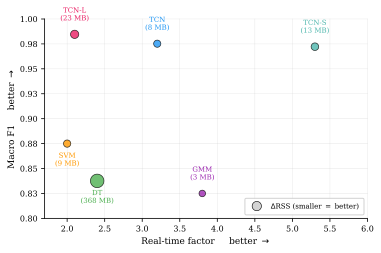
\includegraphics[width=0.94\linewidth]{cpu_benchmark.pdf}\\[2mm]
  Macro F1 against per-frame latency on Intel i5-8300H. Every TCN variant
  stays well below the real-time budget; SVM and GMM exceed it by an order
  of magnitude.
}

\block{Contributions}{
  \begin{itemize}
    \setlength{\itemsep}{2mm}
    \item \textbf{100-hour balanced dataset} for three-class speech/music/background
          classification, published on HuggingFace with a paired adversarial
          critical subset.
    \item \textbf{Faithful re-implementation} of four reference models with
          every deviation documented and motivated.
    \item \textbf{TCN-L hybrid} (delta$^{2}$ frontend + LSTM tail) reaches
          \textbf{0.9846 macro F1} --- the strongest deployed model.
    \item \textbf{TCN-S compact variant}: \textbf{0.9722 macro F1 at
          $\approx$4.6\,K parameters}, \textbf{5.3$\times$ faster than real time on a
          7-year-old laptop CPU} --- a streaming-deployable replacement for the
          classic baselines.
  \end{itemize}
}

\end{columns}

\end{document}
